\documentclass[11pt,a4paper]{article}

\usepackage{../../templates/style}

\begin{document}

\begin{problem}{TOI}{standard input}{standard output}{1 second}{64 megabytes}

การสั่งให้คอมพิวเตอร์ทำงาน โดยพื้นฐานแล้วจำเป็นต้องเขียนเป็นภาษาเครื่องซึ่งเป็นการแทนด้วยเลขฐานสอง แต่การสั่งงานด้วยเลขฐานสองนั้นเป็นการยากที่มนุษย์จะเข้าใจและสั่งให้คอมพิวเตอร์ทำงานได้ถูกต้อง มนุษย์จึงเขียนในภาษาระดับที่สูงขึ้นและแปลเป็นภาษาที่คอมพิวเตอร์เข้าใจด้วย “คอมไพล์เลอร์” ในระบบภาษาอย่างง่ายภาษาหนึ่งซึ่งออกแบบมาเพื่อใช้สอบคอมพิวเตอร์โอลิมปิกในประเทศไทยโดยเฉพาะ ซึ่งภาษานี้มีชื่อว่า “ต๋อย” ซึ่งมาจากภาษาอังกฤษว่า \textit{Thailand Olympiad in Informatics (TOI)} ภาษานี้มีความกะทัดรัดและยังอยู่ในขั้นที่ต้องการปรับปรุงอีกมาก โดยในรุ่นแรกนี้ภาษาต๋อยประกอบด้วย
\begin{enumerate}

\item ข้อความสั่งในการกำหนดค่าตัวแปร
\item ข้อความสั่งในการแสดงค่าตัวแปร
\item การคำนวณเชิงเลขคณิตอย่างง่าย
\end{enumerate}

ซึ่งคำสั่งแต่ละประเภทมีรายละเอียดดังนี้


\begin{figure}[h]
\centering
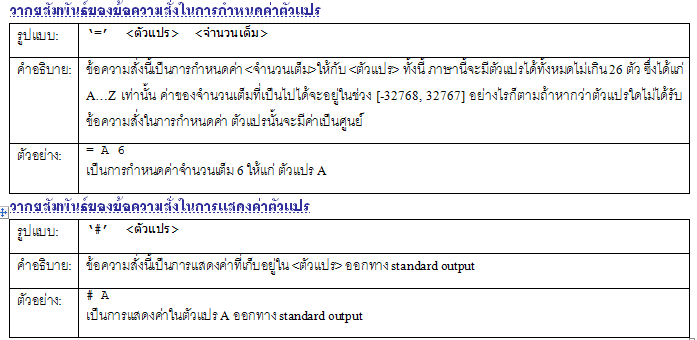
\includegraphics[width=1\textwidth]{../latex/img/1028/1028-1.png}
\end{figure}
\begin{figure}[h]
\centering
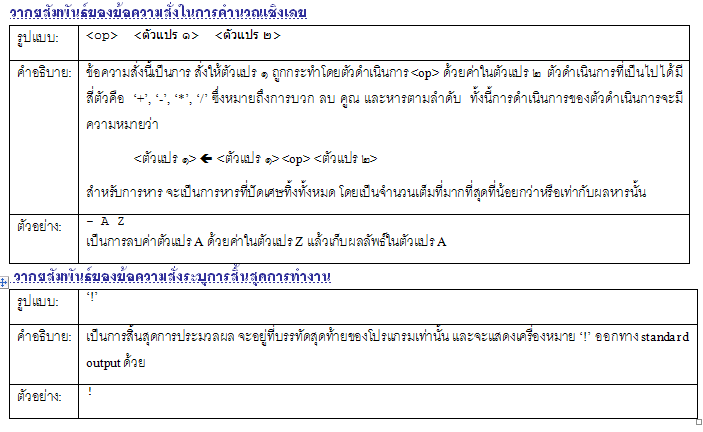
\includegraphics[width=1\textwidth]{../latex/img/1028/1028-2.png}
\end{figure}
\newpage

\textbf{เงื่อนไขอื่นๆของภาษา} ข้อความทั้งหมดเก็บเป็น \textit{ascii} โดยแต่ละบรรทัดจะมีเพียงหนึ่งข้อความสั่งเท่านั้น และบรรทัดว่างจะไม่มีการประมวลผลใดๆ

\bigskip
\underline{\textbf{โจทย์}}  จงเขียนโปรแกรมเพื่อหาผลลัพธ์ของโปรแกรมที่เขียนขึ้นด้วยภาษาต๋อย


\InputFile

\textbf{มีหลายบรรทัด} ข้อมูลนำเข้าจะเป็นโปรแกรมที่เขียนขึ้นด้วยภาษาต๋อย โดยรับผ่านทาง standard input ขนาดของโปรแกรมจะไม่เกินหนึ่งเมกะไบต์ ข้อมูลนำเข้าสำหรับทดสอบทั้งหมดจะถูกเขียนอย่างถูกต้องตามวากยสัมพันธ์ทั้งสิ้น โดยทุกชุดจะมีการแสดงผลลัพธ์บน standard output อย่างน้อยหนึ่งครั้ง ในระหว่างการคำนวณเลขคณิต ชุดทดสอบจะไม่มีผลการคำนวณที่ตัวแปรไม่สามารถเก็บค่าได้ และจะไม่มีการคำนวณที่ต้องการหารค่าด้วยจำนวนเต็มศูนย์


\OutputFile

\textbf{มีหลายบรรทัด} ข้อมูลส่งออกจะแสดงออกที่ standard output ซึ่งเป็นผลลัพธ์การประมวลผลของโปรแกรมภาษาต๋อยที่เป็นข้อมูลนำเข้า

\Examples

\begin{example}
\exmp{= A 1
= B 2
+ A B
\# A
+ A A
\# A
- A B
\# A
* A A
\# A
/ A B
\# A
! }{3
6
4
16
8
!}%
\end{example}


\Source

การแข่งขันคณิตศาสตร์ วิทยาศาสตร์ โอลิมปิกแห่งประเทศไทย สาขาวิชาคอมพิวเตอร์ ประจำปี 2548

\end{problem}

\end{document}